\documentclass[border=10pt]{standalone}

\usepackage[utf8]{inputenc}                                 % Codificação do documento
\usepackage[T1]{fontenc}                                    % Seleção de código de fonte
\usepackage{microtype}                                      % Melhora a justificação do documento
\usepackage{lmodern}                                        % Usa a fonte Latin Modern
\usepackage{ae, aecompl}                                    % Fontes de alta qualidade

\usepackage{amsmath}
\usepackage{verbatim}
\usepackage{tikz}
\usetikzlibrary{arrows,calc,positioning,shadows.blur,decorations.pathreplacing}
\usepackage{etoolbox}

\usepackage{fontawesome}

\begin{document}
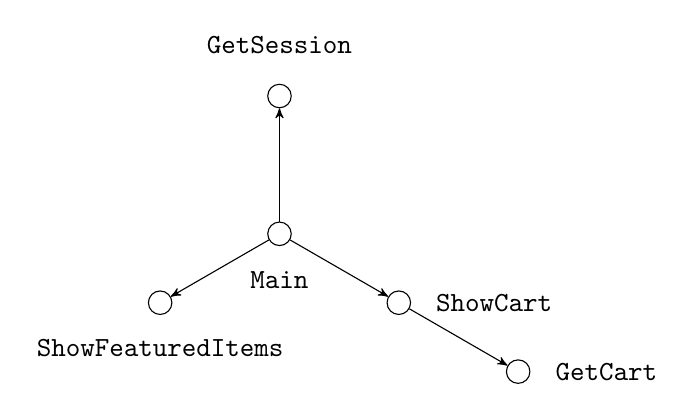
\begin{tikzpicture}
[
                  x =  1.75cm,
	              y = -1.75cm,
	           ->, >= stealth',
	  node distance = 2cm,
	  vertex/.style = { draw=black, circle, inner sep=3pt },
         dot/.style = { draw=black, fill=black, circle, inner sep=0.75pt },
  coordinate/.style = { draw=none, fill=none, circle, inner sep=0pt, outer sep=0pt },
	   label/.style = { draw=none, fill=none, anchor=west },
	toplabel/.style = { draw=none, fill=none, anchor=north }
]

    \node (Main)                at (1, 0)       [vertex] {};
    \node (GetSession)          at (1,-1)       [vertex] {};
    \node (ShowFeaturedItems)   at (0.134, 0.5) [vertex] {};
    \node (ShowCart)            at (1.866, 0.5) [vertex] {};
    \node (GetCart)             at (2.7321, 1)  [vertex] {};

    \draw (Main) -> (GetSession);
    \draw (Main) -> (ShowFeaturedItems);
    \draw (Main) -> (ShowCart);
    \draw (ShowCart) -> (GetCart);

    \node (MainLabel)               at (1, 0.2)     [toplabel] {\texttt{Main}};
    \node (GetSessionLabel)         at (1,-1.5)     [toplabel] {\texttt{GetSession}};
    \node (ShowFeaturedItemsLabel)  at (0.134, 0.7) [toplabel] {\texttt{ShowFeaturedItems}};
    \node (ShowCartLabel)           at (2.066, 0.5) [label]    {\texttt{ShowCart}};
    \node (GetCartLabel)            at (2.9321, 1)  [label]    {\texttt{GetCart}};

\end{tikzpicture}
\end{document}